% twoside = false setzen, falls kein doppelseitiger Druck nötig
\documentclass[oneside, ngerman, final, 11pt, a4paper, 1.1headlines, headinclude=false, footinclude=false, mpinclude=false, pagesize, onecolumn, titlepage, parskip=half, headsepline, chapterprefix=false, version=first, listof=totoc, bibliography=totoc, toc=graduated, fleqn, twoside=true]{scrbook}

% Import file that contains configuration
% Die folgenden Pakete werden in der TEX-Vorlage verwendet.
% Sollten zusätzliche Pakete verwendet werden, sind sie an dieser Stelle hinzuzufügen 
\usepackage[T1]{fontenc}
\usepackage{listings}
\usepackage{refstyle}
\usepackage{float}
\usepackage{textcomp}
\usepackage{graphicx}
\usepackage{nomencl}
\usepackage{textpos} 
\usepackage{xcolor}
\usepackage{tocloft}
\usepackage{lipsum}
\usepackage[utf8]{inputenc}
\usepackage{color}
\usepackage{scrhack}
\usepackage{babel}
\usepackage{wrapfig}

% Custom packages
\usepackage{url}
% to allow the configuration of caption
\usepackage{caption}
\usepackage{hyperref}

\usepackage{tikz}
\usepackage{pgfplots}
% see https://tex.stackexchange.com/questions/1460/script-to-automate-externalizing-tikz-graphics
\usetikzlibrary{external}
\tikzexternalize[prefix=tikz-figures/]
% see https://tex.stackexchange.com/questions/7953/how-to-expand-texs-main-memory-size-pgfplots-memory-overload
\usepgfplotslibrary{external}

\usepackage{tabularx}
\usepackage{makecell}
\usepackage{csquotes}

% allow rotation of boxes (like a table)
% see https://tex.stackexchange.com/a/133744/221944
\usepackage{hvfloat}

% see https://tex.stackexchange.com/a/26483/221944
\usepackage{longtable}

% Import file that contains configuration


% Schachtelungstiefe eine Nummerierung der Überschriften 
\setcounter{secnumdepth}{3}
\setcounter{tocdepth}{3}

% Die folgenden Befehle sind nüzulich bei Verwendung des alten nomencl.sty Pakets
\providecommand{\printnomenclature}{\printglossary}
\providecommand{\makenomenclature}{\makeglossary}
\makenomenclature

% Zusätzliche Konfigurationen 
\makeatletter
\setkomafont{disposition}{\normalcolor\bfseries}
\makeatother

% Custom Zeugs

% Umbenennen von Listings und Nomenklatur 
\renewcommand{\nomname}{Abkürzungs- und Erklärungsverzeichnis}
\renewcommand\lstlistlistingname{Quellcodeverzeichnis}
\renewcommand{\lstlistingname}{Quellcode}
\renewcommand\appendixname{Anhang}

\addto\captionsngerman{
	\renewcommand{\figurename}{Abb.\@}
	\renewcommand{\tablename}{Tab.\@}
}

% Listing defintion for JavaScript and ECMAScript2015 (ES6)
%
% ECMAScript 2015 (ES6) definition by Gary Hammock
%

\lstdefinelanguage[ECMAScript2015]{JavaScript}[]{JavaScript}{
	morekeywords=[1]{await, async, case, catch, class, const,
		default, do, enum, export, extends, finally, from, implements,
		import, instanceof, let, static, super, switch, throw, try},
	morestring=[b]` % Interpolation strings.
}


%
% JavaScript version 1.1 by Gary Hammock
%
% Reference:
%	 B. Eich and C. Rand Mckinney, "JavaScript Language Specification
%		 (Preliminary Draft)", JavaScript 1.1.	1996-11-18.	[Online]
%		 http://hepunx.rl.ac.uk/~adye/jsspec11/titlepg2.htm
%

\lstdefinelanguage{JavaScript}{
	morekeywords=[1]{break, continue, delete, else, for, function,
		if, in, new, return, this, typeof, var, void, while, with, =>,
		constructor, window, class, interface, enum, declare, const,
		var, typeof},
	% Literals, primitive types, and reference types.
	morekeywords=[2]{false, null, true, boolean, number, undefined,
		Array, Boolean, Date, Math, Number, String, Object, void, any,
		string, private, public, protected},
	% Built-ins.
	morekeywords=[3]{eval, parseInt, parseFloat, escape, unescape,
		pipe, tap, subscribe},
	morekeywords=[4]{@Injectable, @NgModule, @Inject},
	sensitive,
	morecomment=[s]{/*}{*/},
	morecomment=[l]//,
	morecomment=[s]{/**}{*/}, % JavaDoc style comments
	morestring=[b]',
	morestring=[b]"
}[keywords, comments, strings]


\lstalias[]{ES6}[ECMAScript2015]{JavaScript}

% Requires package: color.
\definecolor{mediumgray}{rgb}{0.3, 0.4, 0.4}
\definecolor{mediumblue}{rgb}{0.0, 0.0, 0.8}
\definecolor{forestgreen}{rgb}{0.13, 0.55, 0.13}
\definecolor{darkviolet}{rgb}{0.58, 0.0, 0.83}
\definecolor{royalblue}{rgb}{0.25, 0.41, 0.88}
\definecolor{crimson}{rgb}{0.86, 0.8, 0.24}

\lstdefinestyle{JSES6Base}{
	backgroundcolor=\color{white},
	basicstyle=\ttfamily,
	breakatwhitespace=false,
	breaklines=true,
	captionpos=b,
	columns=fullflexible,
	commentstyle=\color{mediumgray}\upshape,
	emph={},
	emphstyle=\color{crimson},
	extendedchars=true,	% requires inputenc
	fontadjust=true,
	frame=single,
	identifierstyle=\color{black},
	keepspaces=true,
	keywordstyle=\color{mediumblue},
	keywordstyle={[2]\color{darkviolet}},
	keywordstyle={[3]\color{royalblue}},
	keywordstyle={[4]\color{mediumblue}},
	numbers=left,
	numbersep=5pt,
	numberstyle=\color{black},
	rulecolor=\color{black},
	showlines=true,
	showspaces=false,
	showstringspaces=false,
	showtabs=false,
	stringstyle=\color{forestgreen},
	tabsize=2,
	title=\lstname,
	upquote=true,	% requires textcomp
	literate={ä}{{\"a}}1 {ö}{{\"o}}1 {ü}{{\"u}}1 {Ä}{{\"A}}1 {Ö}{{\"O}}1 {Ü}{{\"U}}1 {ß}{{\ss}}1,
}

\lstdefinestyle{JavaScript}{
	language=JavaScript,
	style=JSES6Base
}
\lstdefinestyle{ES6}{
	language=ES6,
	style=JSES6Base
}

% Listing defintion for Java
% Farben fuer Programmlisting
\usepackage{listings,xcolor}
\definecolor{pl_background}{rgb}{0.95,0.95,0.95}
\definecolor{pl_comment}{rgb}{0.12, 0.38, 0.18 }
\definecolor{pl_ifelse}{rgb}{0.74,0.74,.29}
\definecolor{pl_keyword}{rgb}{0.37, 0.08, 0.25}
\definecolor{pl_string}{rgb}{0.06, 0.10, 0.98}

\definecolor{lstbackground}{RGB}{235,235,235}
\definecolor{lstkeyword}{RGB}{127,0,85}
\definecolor{lststring}{RGB}{42,0,255}
\definecolor{lstcomment}{RGB}{63,127,95}
\definecolor{lstannotation}{RGB}{127,159,191}

\definecolor{fh_grau}{rgb}{0.76,0.75,0.76}

% Vordefiniertes Programmlisting
\lstset{
	basicstyle = \small\sffamily,
	backgroundcolor = \color{pl_background},
	stringstyle = \color{pl_string},
	keywordstyle = \color{pl_keyword}\bfseries,
	commentstyle = \color{pl_comment}\itshape,
	frame = lrbt,
	numbers = left,
	captionpos=b,
	showstringspaces = false,
	breaklines = true,
	xleftmargin = 15pt,
	emph = [1]{php},
	emphstyle = [1]\color{black},
	emph = [2]{if,and,or,else},
	emphstyle = [2]\color{pl_ifelse}
}

% Quellcde Formatierung im normalen Stil 
\lstset{
	basicstyle={\footnotesize\fontfamily{pcr}\selectfont},
	backgroundcolor=\color{lstbackground},
	breaklines=true,
	frame=single,
	numbers=left,
	showstringspaces=false,
	tabsize=4
}

% Quellcde Formatierung im Eclipse Stil
\lstdefinestyle{java-eclipse}{
	commentstyle={\color{lstcomment}},
	keywordstyle={\color{lstkeyword}\bfseries},
	stringstyle={\color{lststring}},
	moredelim={[il][\textcolor{lstannotation}]{§§}},
	moredelim={[is][\textcolor{lstannotation}]{\%\%}{\%\%}}
}

% own commands
\newcommand{\etal}{\textit{et al.\@ }}
\newcommand{\citationneeded}{{\color{red}[cite]}}
\newcommand{\source}[1]{\vspace{-0.75\baselineskip}\caption*{Quelle: {#1}} }

\newcounter{anfcounter}
\renewcommand{\theanfcounter}{\arabic{anfcounter}}

\makeatletter
\newenvironment{anf}[6]{%
\refstepcounter{anfcounter}%
\protected@edef\@currentlabel{Anforderung #2}
\label{#1}%
	\begin{table}[H]
	\begin{tabular}{ |p{1.25cm}|p{5.5cm}|p{2.25cm}|p{2.1cm}|p{1.25cm}| }
\hline
Id   & Name          & Kano-Modell  & Funktionsart & Quelle       \\
#2 & #3 & #4 & #5 & #6 \\
\hline
}%
{
	\end{tabular}
	\end{table}%
}%
\makeatother

% allow breaking of urls
% see https://tex.stackexchange.com/a/344711/221944
\def\UrlBreaks{\do\/\do-}

\newcommand*\circled[1]{
	\tikz[baseline=(char.base)]{
		\node[shape=circle,draw,inner sep=2pt] (char) {#1};
	}
}

\pgfplotsset{compat=1.17}

% Gherkin
% https://gist.github.com/nsommer/9a04f6ebc6ea8b9f5b816becb97e7d9b
\lstdefinelanguage{gherkin}{
	morekeywords = {
		Given,
		When,
		Then,
		And,
		Scenario,
		Feature,
		But,
		Background,
		Scenario Outline,
		Examples
	},
	sensitive=true,
	morecomment=[l]{\#},
	morestring=[b]",
	morestring=[b]',
	% fix umlaute causing issues
	% https://tex.stackexchange.com/questions/24528/having-problems-with-listings-and-utf-8-can-it-be-fixed/24529
	extendedchars=true,
	literate={ä}{{\"a}}1 {ö}{{\"o}}1 {ü}{{\"u}}1 {Ä}{{\"A}}1 {Ö}{{\"O}}1 {Ü}{{\"U}}1 {ß}{{\ss}}1,
}

%\usepackage{glossaries}
%\makeglossaries

\newglossaryentry{Bug Report}
{
    name=Bug Report,
    description={Fehlerbericht},
    plural={Bug Reports},
}


% Beginn des Dokumentes 
\begin{document}
	% Die Commands werden auf der Titelseite eingefügt, die Werte sind anzupassen
	\newcommand*{\thedockind}{Bachelorthesis}
	\newcommand*{\thetitle}{Nachvollziehbarkeit von Nutzerinteraktion und Anwendungsverhalten am Beispiel JavaScript-basierter Webapplikationen}
	\newcommand*{\thesubtitle}{}
	\newcommand*{\theauthor}{Marvin Kienitz}
	\newcommand*{\thematriculationnumber}{7097533}
	\newcommand*{\thebirthday}{26.04.1996}
	\newcommand*{\thedegree}{Bachelor of Science}
	\newcommand*{\themajor}{Software- und Systemtechnik, Vertiefung Softwaretechnik} % Studiengang
	\newcommand*{\thedate}{\today} % \today kann durch ein Datum erstetzt werden. 
	\newcommand*{\thebetreuer}{Prof. Dr. Sven Jörges} 
	\newcommand*{\thezweitbetreuer}{Dipl. Inf. Stephan Müller}

	\begin{titlepage}
	  \begin{textblock}{6.5}(-1,-3)
	    \begin{color}{fh_grau}
	      \rule{6.8cm}{33cm}    
	    \end{color}
	  \end{textblock}
	  \begin{textblock}{6.5}(-1.2,-0.7)
	  \end{textblock}
	  \begin{textblock}{6.5}(-0.8,1)
	    {\Large \textsf{\thedockind}}            
	  \end{textblock}
	
	  \begin{textblock}{6}(4.5,2)
	    {\noindent \huge 
	      \textsf{\textbf{\thetitle\\[0.3cm] 
	          \Large  \thesubtitle\\[0.05cm]
	          }} }
	  \end{textblock}
	
	
	  \begin{textblock}{8.5}(4.5,6.5)\noindent
	    \textsf{An der Fachhochschule Dortmund\\
	    im Fachbereich Informatik\\
	    Studiengang \themajor \\
	    erstellte \thedockind \\
	    zur Erlangung des akademischen Grades\\
	    \thedegree}
	  \end{textblock}
	
	  \begin{textblock}{6.5}(-0.4,10.0)
	    \noindent
	    \textsf{von \\
	      \theauthor \\
	      geb.\ am \thebirthday  \\
	      Matr.-Nr. \thematriculationnumber\\[0.7cm]
	      Betreuer:\\
	       \noindent\hspace*{6mm} \thebetreuer \\
	       \noindent\hspace*{6mm} \thezweitbetreuer\\ [0.5cm]
	      Dortmund, \today}    
	  \end{textblock}
		
	
	\end{titlepage}
	
	\newpage{}
	
	\section*{\thispagestyle{empty}Kurzfassung}
	
	\textit{\lipsum[1-4]}
	
	\newpage{}
	
	\section*{\thispagestyle{empty}Abstract}
	
	\textit{\lipsum[1-4]}
	
	\newpage{}
	
	% Römische Nummerierung der Seiten des Inhaltsverzeichnisses 
	\setcounter{page}{1}
	\pagenumbering{roman}
	
	\tableofcontents{}
	
	\newpage{}
	
	% Arabische Nummerierung aller anderen Seiten
	\setcounter{page}{1} 
	\pagenumbering{arabic}
	
	\chapter{Einleitung}
	% a hack, to make the Motivation fit into one page..
\vspace{-\baselineskip}

%In diesem Unterkapitel sollten folgende Punkte behandelt werden:
%\begin{itemize}
%	\item	Was ist das Problem
%	\item 	Problemgeschichte?
%\end{itemize}
\section{Motivation}

Die Open Knowledge GmbH ist als branchenneutraler Softwaredienstleister in einer Vielzahl von Branchen wie Automotive, Logistik, Telekommunikation und Versicherungs- und Finanzwirtschaft aktiv. Zu den zahlreichen Kunden der Open Knowledge GmbH gehört auch ein führender deutscher Direktversicherer. 

Ein Direktversicherer bietet Versicherungsprodukte seinen Kunden ausschließlich im Direktvertrieb, d. h. vor allem über das Internet und zusätzlich auch über Telefon, Fax oder B
rief an. Im Unterschied zum klassischen Versicherer verfügt ein Direktversicherer jedoch über keinen Außendienst oder Geschäftsstellen, bei denen Kunden eine persönliche Beratung bekommen können. Da das Internet der primäre Vertriebskanal ist, gehört heute ein umfassender Online-Auftritt zum Standard. Dieser besteht typischerweise aus einem Kundenportal mit der Möglichkeit Angebote für Versicherungsprodukte berechnen und abschließen zu können, sowie persönliche Daten und Verträge einzusehen.

\nomenclature[Fachbegriff]{Serverseitiges Rendering}{Die darzustellenden Inhalte, werden beim Server generiert und der Client stellt diese dar. Beispielsweise sind Anwendungen mit PHP oder auch eine Java Web Application}
\nomenclature[Fachbegriff]{Clientseitiges Rendering}{Der Server stellt dem Client lediglich die Logik und die notwendigen Daten bereit, die eigentliche Inhaltsgenerierung geschieht im Client. Für ein Beispiel siehe \autoref{subsec:singe-page-applications}}

% i.d.R. getrennt: https://www.scribbr.de/wissenschaftliches-schreiben/abkuerzungen/
Während in der Vergangenheit Online-Auftritte i. d. R. als Webapplikation mit serverseitigen Rendering realisiert wurden, sind heutzutage Javascript-basierte Webapplikation mit clientseitigem Rendering die Norm. Bei einer solchen Webapplikation befindet sich die gesamte Logik mit Ausnahme der Berechnung des Angebots und der Verarbeitung der Antragsdaten im Browser des Nutzers.

Im produktiven Einsatz kommt es auch bei gut getesteten Webapplikationen hin und wieder vor, dass es zu unvorhergesehenen Fehlern in der Berechnung oder Verarbeitung kommen kann. Liegt die Ursache für den Fehler im Browser, z. B. aufgrund einer ungültigen Wertkombination, ist dies eine Herausforderung. Während bei Server-Anwendungen Fehlermeldungen in den Log-Dateien einzusehen sind, gibt es für den Betreiber der Anwendung i. d. R. keine Möglichkeit die notwendigen Informationen über den Nutzer und seine Umgebung abzurufen. Noch wichtiger ist, dass er mitbekommt, wenn ein Nutzer ein Problem bei der Bedienung der Anwendung hat. Ohne eine aktive Benachrichtigung durch den Nutzer, sowie detaillierte Informationen, ist es dem Betreiber nicht möglich, Kenntnis über das Problem zu erlangen, geschweige denn dieses nachzustellen.

Dies stellt ein Kernproblem von  Webapplikationen dar \cite{ClientSideMonitoringOfDistributedSystems}. Im Rahmen der Arbeit soll daher ein Proof-of-Concept konzipiert und umgesetzt werden, welcher dieses Kernproblem am Beispiel einer Demoanwendung löst.

%\begin{itemize}
%	\item 	Was soll mit der Arbeit erreicht werden? Welche Ziele werden angestrebt?
%			Möglichst kurz und präzise geplante Ergebnisse umreißen. Daran werden
%			Ihre Resultate am Ende gemessen!
%\end{itemize}
\section{Zielsetzung}

Das grundlegende Ziel dieser Arbeit soll es sein, den Betreibern einer JavaScript-basierten Webapplikation die Möglichkeit zu geben das Verhalten ihrer Applikation und die Interaktionen von Nutzern in speziellen Situationen nachzuvollziehen. Diese speziellen Situationen sollen sich auf Fehlerfälle und für die Betreiber interessante Situationen konzentrieren, die jeweils einen Auslösepunkt in der Applikation haben. Eine vollständige Überwachung der Applikation und des Nutzers (wie bpsw. bei Werbe-Tracking) sind nicht vorgesehen. Es sollen keine detaillierten Erfahrungen in der Webentwicklung vom Leser erwartet werden. Damit dies gewährleistet werden kann, ist unter anderem das Projektumfeld und seine besonderen Eigenschaften zu erklären.

Die anzustrebende Lösung soll ein Proof-of-Concept sein, welches anhand einer bestehenden Demo-Anwendung erstellt werden soll. Die Demo-Anwendung soll repräsentativ eine abgespeckte JavaScript-basierte Webapplikation darstellen, bei der die zuvor benannten Hürden zur Nachvollziehbarkeit bestehen.

Vor der eigentlichen Lösungserstellung soll jedoch die theoretische Seite beleuchtet werden, indem die Nachvollziehbarkeit sowie Methoden und Praktiken zur Erreichung dieser beschrieben werden. Es gilt aktuelle Literatur und den Stand der Technik zu erörtern, in Bezug auf die Forschungsfrage. Beim Stand der Technik sollen zwei bis drei Technologien näher betrachtet werden und beschrieben werden.

Weiterhin gilt es zu beleuchten, wie die Auswirkungen für die Nutzer der Webapplikation sind. Wurde die Leistung der Webapplikation beeinträchtigt (erhöhte Ladezeit, erhöhte Datenlast)? Werden mehr Daten von ihm erhoben und zu welchem Zweck (Stichwort DSGVO)?

Am Ende der Ausarbeitung soll überprüft werden, ob und wie die Forschungsfrage beantwortet wurde. Auch die Übertragbarkeit der erstellten Lösung (PoC) und Ergebnisse gilt es hierbei näher zu betrachten.

\subsection{Abgrenzung}

\nomenclature[Fachbegriff]{PoC}{Proof-of-Concept}

Bei der Betrachtung von Webapplikationen, wird sich auf Single-Page-Applications (SPAs) konzentriert, denn hier bewegt sich das Projektumfeld von der Open Knowledge GmbH. Bei der Betrachtung der Datenerhebung und -verarbeitung ist eine volle Konformität mit der DSGVO nicht zu prüfen.

Bei der Erörterung zum Stand der Technik sollen detaillierte Produktvorstellungen nicht das Ziel sein, auch ist keine umfassende Gegenüberstellung anzustreben.

\pagebreak

%\begin{itemize}
%	\item 	Wie wird vorgegangen, um das Ziel zu erreichen?
%	\item 	Warum ist die Arbeit so gegliedert, wie sie gegliedert ist?
%	\item 	Welche Aspekte werden nicht behandelt und warum?
%\end{itemize}
\section{Vorgehensweise}

Zur Vorbereitung eines Proof-of-Concepts wird zunächst die Ausgangssituation geschildert. Speziell wird auf die Herausforderungen der Umgebung ``Browser`` eingegangen, besonders in Hinblick auf die Verständnisgewinnung zu Interaktionen eines Nutzers und des Verhaltens der Applikation. Des Weiteren wird die Nachvollziehbarkeit als solche formal beschrieben und was sie im Projektumfeld genau bedeutet.

% Um das Ziel, die Erstellung eines Proof-of-Concept (PoC), zu erreichen, wird vorerst die Literatur geprüft und die Ausgangssituation erörtert und beschrieben. Die Nachvollziehbarkeit und ihr Nutzen werden vorgestellt.

%Es ist dem Leser zu vermitteln, was die theoretischen Grundlagen sind und wie die der Nachvollziehbarkeit definiert wird. Es gilt zu erörtern, warum die Nachvollziehbarkeit erstrebenswert ist und wie sehr sie bereits Beachtung findet.

Darauf aufbauend werden allgemeine Methoden vorgestellt, mit der die Stakeholder eine bessere Nachvollziehbarkeit erreichen können. Dabei werden die Besonderheiten der Umgebung beachtet und es wird erläutert, wie diese Methoden in der Umgebung zum Einsatz kommen können.

% Durch das gewonnene Verständnis über die Ausgangssituation, werden nun Methoden aufgezeigt, welche eine Nachvollziehbarkeit unterstützen. Methoden wie Fehlerberichte, Logging, Monitoring und ggf. andere sind zu betrachten.

Auf Basis des detaillierten Verständnisses der Problemstellung und der Methoden wird nun ein Proof-of-Concept erstellt. Ziel soll dabei sein, die Nachvollziehbarkeit einer Webapplikation zu verbessern. Der Proof-of-Concept erfolgt auf Basis einer Demo-Anwendung, die im Rahmen dieser Arbeit erstellt wird.

Ist ein Proof-of-Concept nun erstellt, wird analysiert, welchen Einfluss es auf die Nachvollziehbarkeit hat und ob die gewünschten Ziele erreicht wurden (vgl. Zielsetzung).

% Anfangs soll identifiziert werden, was alles für einen Nutzer ein Problem darstellen kann. Es muss sich bei den Problemen nicht nur um Laufzeitfehler o.Ä. handeln, sondern Logikfehler oder auch Verständnisprobleme führen zu einer Einschränkung der Nutzbarkeit. Hier soll eine Analyse aus der Literatur und ggf. einer Umfrage erstellt werden, um daraufhin grobe Problembilder zu klassifizieren.

% Danach soll erörtert werden, welche Ursachen es für häufige Problemszenarien gibt. Darauf aufbauend könnten Aussagen getroffen werden, wie diese Szenarien bereits vorher vermeidet werden können oder die Häufigkeit reduziert werden kann.

%Durch das gewonnene Verständnis über diese Probleme, soll nun ein Konzept erarbeitet werden. Dieses Konzept soll darauf abzielen zu den einzelnen Problembildern jeweils einen Ansatz zu finden, diese aufzuzeigen und den Stakeholdern Informationen zu liefern, die bei der Behebung notwendig sind (bspw. Geräteinformationen, Sitzungsinformationen, Logs, etc.).

% Zunächst soll ein Konzept erstellt werden, welches die Komponenten definiert und beschreibt und die Interaktion zwischen den Komponenten umfasst. Auf Basis der Konzeptes soll nun die Implementierung der Erweiterung erfolgen.

% Da nun ein Basisverständnis gewonnen wurde, sollen etablierte Technologien wie Google Cloud \cite{GoogleCloudErrorReporting}, Dynatrace \cite{DynatraceDigitalExperienceMonitoring}, Sentry \cite{SentryForJavaScript} und LogRocket \cite{LogRocket} näher betrachtet werden. Durch die Erörterung des Stands der Technik sollen folgend Empfehlungen ausgesprochen werden, für welche Projekte welche Technologie oder Kombination von Technologien sinnvoll ist. Sollte keine Technologie als angemessen betrachtet werden, so soll basierend auf den Anforderungen ein Vorschlag gemacht werden, wie so eine Technologie aussehen könnte.

%\newpage

\section{Open Knowledge GmbH}

%{\color{red}TODO: Dieser Abschnitt muss noch überarbeitet werden}

Die Bachelorarbeit wird im Rahmen einer Werkstudententätigkeit innerhalb der Open Knowledge GmbH erstellt. Der Standortleiter des Standortes Essen, Dipl. Inf. Stephan Müller, übernimmt die Zweitbetreuung.

Die Open Knowledge GmbH ist ein branchenneutrales mittelständisches Dienstleistungsunternehmen mit dem Ziel bei der Analyse, Planung und Durchführung von Softwareprojekten zu unterstützen. Das Unternehmen wurde im Jahr 2000 in Oldenburg, dem Hauptsitz des Unternehmens, gegründet und beschäftigt heute 74 Mitarbeiter. Mitte 2017 wurde in Essen der zweite Standort eröffnet, an dem 13 Mitarbeiter angestellt sind.

Die Mitarbeiter von Open Knowledge übernehmen in Kundenprojekten Aufgaben bei der Analyse über die Projektziele und der aktuellen Ausgangssituationen, der Konzeption der geplanten Software, sowie der anschließenden Implementierung. Die erstellten Softwarelösungen stellen Individuallösungen dar und werden den Bedürfnissen der einzelnen Kunden entsprechend konzipiert und implementiert. Technisch liegt die Spezialisierung bei der Mobile- und bei der Java Enterprise Entwicklung, bei der stets moderne Technologien und Konzepte verwendet werden. Die Geschäftsführer als auch diverse Mitarbeiter der Open Knowledge GmbH sind als Redner auf Fachmessen wie der Javaland oder als Autoren in Fachzeitschriften wie dem Java Magazin vertreten. % Aufgrund der großen Expertise in den Bereichen Technologien und Konzepte sind sowohl die Geschäftsführer als auch diverse Mitarbeiter der Open Knowledge GmbH als Redner auf Fachmessen wie der Javaland oder Autoren in Fachzeitschriften wie dem Java Magazin vertreten.% \cite{VincentOpenKnowledge} % Auch aufgrund der medialen Präsenz konnte die Open Knowledge GmbH in den letzten Jahre zahlreiche Projekte für namhafte Kunden, wie z. B. Vodafone, die HUK-Coburg, die Daimler AG und die DB Schenker AG übernehmen. \cite{VincentOpenKnowledge}

%Durch das breite Dienstleistungsangebot und die Branchenneutralität übernimmt die Open Knowledge GmbH Projekte aus der Automobilindustrie, der Luft- und Raumfahrt, dem Bankwesen und dem Versicherungswesen innerhalb des nationalen und europäischen Raums.
%
%Entsprechend der Philosophie ``Offenkundig Gut`` und dem Namen des Unternehmens wird stets versucht das benötigte Wissen zur Erstellung und Wartung der Software mit dem Kunden zu teilen, sodass die Kunden nach Abschluss der Projekte in der Lage sind, die Software selbstständig zu Pflegen und die Projektarbeit von OK damit abgeschlossen ist \cite{OpenKnowledgePhilosophie}.

\pagebreak

	
	\chapter{Instandhaltung und Support}
	% \chapter{Instandhaltung und Support}

\section{Phase in Softwareprojekten}

	\begin{wrapfigure}[14]{r}{0.45\linewidth}
		\centering
		\vspace{-\baselineskip}
		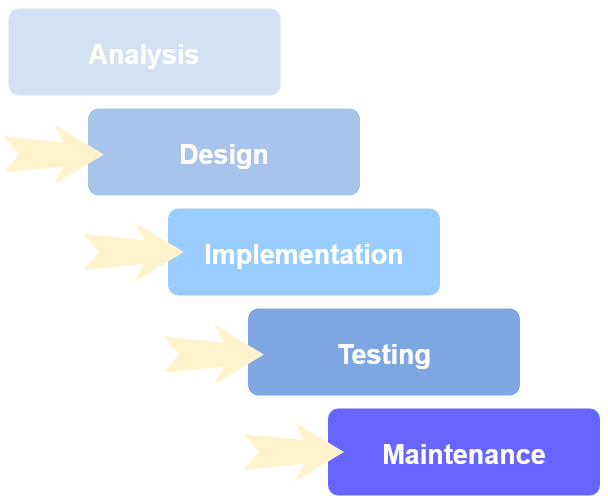
\includegraphics[width=\linewidth]{img/02_maintenance/software-life-cycle.png}
		\caption{Lebenszyklus einer Software}
		\label{fig:software-development-life-cycle}
		\source{Eigene Darstellung von \cite{ASimulationModelWaterfallSoftware}}
	\end{wrapfigure}
	
	In vielen Modellen über den Lebenszyklus einer Software gibt es eine Phase, in der Instandhaltung und Support den Alltag bestimmen, sie wird oftmals ``Maintenance`` bezeichnet \cite{ManagingTheComplexityOfWebSystemsDevelopment} \cite{ASimulationModelWaterfallSoftware}. Sie ist nach Zelkowitz \etal \cite{PrinciplesOfSoftwareEngineeringAndDesign} für rund zwei Drittel der Entwicklungskosten verantwortlich, begründet durch exponentielle Steigung \cite{ExtremeProgrammingExplained}.
	
	Es werden immer bessere Methoden entwickelt, um Probleme in Software - oder auch Bugs - zu verringern. Jedoch erhöht sich zugleich die Komplexität von Software, was zur Ursache hat, dass es mehr Nährboden für Bugs gibt \cite{TrackingDownSoftwareBugsAnomalyDetection}. De-facto sind Bugs ein unvermeidbarer Bestandteil einer Software und müssen daher erwartet und gehandhabt werden \cite{TheMythicalManMonth}.
	
	Wenn nun ein Bug auffällt, sei es durch einen Nutzer oder auch zufällig einem Stakeholder, muss entschieden werden, ob dieser zu beheben ist. Wenn eine Behebung angestrebt wird, benötigt der Stakeholder meistens Rahmeninformationen \citationneeded um den Bug ggf. zu reproduzieren und die Situation \textbf{nachzuvollziehen}. Desto mehr Verständnis der Stakeholder über das Problem erhält, desto schneller und präziser kann er die Ursache aufdecken. Die Ermöglichung der schnellen Verständnis über ein Problem, wird in dieser Arbeit Nachvollziehbarkeit genannt.

\section{Nachvollziehbarkeit}

	Sie beschäftigt sich mit der Informationserfassung und -aufbereitung, um das Verhalten eines Systems und die Interaktionen der Nutzer verstehen zu können.

\section{Maintenance bei Webapplikationen}

	\textit{Hier sollen die Besonderen Hürden bei Webapplikationen hervorgehoben werden (ungeschulte Nutzer, indirekte Kommunikation, etc.)}
	
	\chapter{Methoden und Praktiken}
	% \chapter{Methoden und Praktiken}

\textit{In diesem Kapitel soll beschrieben werden, wie eine Nachvollziehbarkeit in Webapplikationen erreicht werden kann. Spezielle Methoden und Praktiken sollen vorgestellt und beleuchtet werden.}
% \textit{Hier könnte unter anderem \textbf{OpenTelemetry} betrachtet werden.}

\section{Methoden}

\subsection{Logging}

\textit{Folgende Fragen sollen zur Methode beantwortet werden}
\begin{enumerate}
	\item \textit{Gibt es Besonderheiten zu Logging in anderen Projekten (Backend vs. Frontend)?}
	\item \textit{Wie können Logs an einen auswertenden Stakeholder gelangen?}
	\item \textit{Welches Verhalten kann hiermit aufgedeckt/nachvollziehbar gemacht werden?}
\end{enumerate}

%\subsection{Monitoring}
%
%\textit{Folgende Fragen sollen zur Methode beantwortet werden}
%\begin{enumerate}
%	\item \textit{Welche Anwendungseigenschaften sind zu monitoren?}
%	\item \textit{Welches Verhalten kann hiermit aufgedeckt/nachvollziehbar gemacht werden?}
%\end{enumerate}

\subsection{Metriken}

\textit{Folgende Fragen sollen zur Methode beantwortet werden}
\begin{enumerate}
	\item \textit{Welche Metriken können definiert?}
	\item \textit{Wie können Metriken definiert werden?}
	\item \textit{Welches Verhalten kann hiermit aufgedeckt/nachvollziehbar gemacht werden?}
\end{enumerate}

\subsection{Tracing}

\textit{Folgende Fragen sollen zur Methode beantwortet werden}
\begin{enumerate}
	\item \textit{Welche Nutzerinteraktionen sind zu tracen?}
	\item \textit{Welches Verhalten kann hiermit aufgedeckt/nachvollziehbar gemacht werden?}
\end{enumerate}

\subsection{Fehlerberichte}

\textit{Folgende Fragen sollen zur Methode beantwortet werden}
\begin{enumerate}
	\item \textit{Was genau sind Fehlerberichte (=Bug-Reports) }
	\item \textit{Welches Verhalten kann hiermit aufgedeckt/nachvollziehbar gemacht werden?}
\end{enumerate}

\section{Praktiken aus der Fachpraxis}

\textit{Neben den allgemeinen Methoden weisen einige Technologien in sich geschlossene Funktionsbereiche auf, die einen eigenen Ansatz darstellen. Diese Ansätze sollen hier getrennt von der jeweiligen Technologie beschrieben werden. (Beispielsweise ``Real User Monitoring``)}

\section{Werkzeuge und Technologien}

\textit{Basierend auf dem Grundwissen über die Methoden und Praktiken, soll nun der Stand der Technik aus Fachpraxis und Literatur erörtert werden. Hierbei sollen Werkzeuge und Technologien und ihre Ansätze hervorgehoben werden und mit Hilfe welcher Methoden sie welches Ziel erreichen.}

\textit{In diesem Abschnitt werden die Technologien vom Autor evaluiert und dann beschrieben. Es soll jedoch keine Gegenüberstellung erfolgen, sondern einfach eine Evaluierung, dieses Wissen soll dann später in der Erstellung des Lösungsansatzes helfen.}

\textit{Weiterhin könnte beleuchtet werden, wie ähnliche Herausforderungen bei anderen „Fat-Client“-Lösungen (also nicht SPAs) angegangen werden, und ob man hier etwas lernen oder übertragen kann (und wenn nicht, warum nicht)?}

\section{Fachpraxis}

\textit{Eine geringe Menge (3-8) an Technologien soll hierbei evaluiert werden, im Idealfall durch praktischen Einsatz.}

\section{Literatur}

\begin{enumerate}
	\item \textit{Gibt es hierzu Ansätze in der Literatur?}
	\item \textit{Wie sehen diese aus, welchen Zweck erfüllen sie?}
	\item \textit{Sind sie vergleichbar mit Ansätzen aus der Fachpraxis?}
\end{enumerate}
	
	\chapter{Beispielhafte Integration}
	% \chapter{Beispielhafte Integration}
	
\section{Vorstellung der Demoanwendung}

	\textit{In diesem Abschnitt soll die Demoanwendung vorgestellt werden, anhand dessen das Proof-of-Concept erstellt wird. Damit das Proof-of-Concept erstellt werden kann, muss die Demoanwendung die zuvor beschriebenen Probleme aufweisen, hierbei sollen die Probleme möglichst realitätsnah sein und nicht frei erfunden.}
	
\section{Konzept}
	
	\subsection{Architektur}

	\textit{Hier soll die grobe Architektur geplant werden, welche Komponente es gibt und wie diese kommunizieren sollen.}
	
	\subsection{Datenverarbeitung}
		
		\subsubsection{Erhebung}
		\textit{Wie werden die Daten erhoben (Nennung der verwendeten Methoden!)?}
		\textit{Wie gelangen die Daten an eine auswertende Komponente?}
		
		\subsubsection{Auswertung}
		\textit{Wie werden die Daten zusammengefasst und ausgewertet?}
		\textit{Wie gelangt das Ergebnis an die darstellende Komponente?}
		
		\subsubsection{Visualisierung}
		\textit{Wie werden den Stakeholdern die Informationen präsentiert?}

\section{Implementierung}

	\textit{Auf Basis des Konzeptes soll nun eine Implementierung erfolgen.}

	\subsection{Technologie-Stack}

\section{Demonstration}

	\textit{Nachdem nun eine Implementierung steht, soll die Erweiterung auf nicht-technische Weise veranschaulicht werden. Hier soll dargestellt werden, wie die Nachvollziehbarkeit nun verbessert worden ist.}
	
	\chapter{Abschluss}
	% \chapter{Abschluss}

\section{Fazit}
\textit{\lipsum[1]}

\section{Ausblick}
\textit{\lipsum[1]}
	
%	\chapter{Test-Kapitel}
%	\section{Zitate}

Im Literaturverzeichnis sollte zu jedem Zitat ein Eintrag mit dem entsprechenden Kürzel zu finden sein.

\subsection{Einzelner Autor}

Zur Überprüfung wird das Buch \enquote{The Hitchhiker's Guide to the Galaxy}  von Douglas Adams aus dem Jahr 1979 hinzugezogen. Die folgende Zitierung sollte mit \texttt{[Ada79]}  abgekürzt dargestellt werden. \textit{Zitat} \cite{TestCitation001}.

\subsection{Zwei Autoren}

Zur Überprüfung wird das Buch \enquote{Hard drive: Bill Gates and the making of the Microsoft empire} von James Wallace und Jim Erickson aus dem Jahr 1992 hinzugezogen. Die folgende Zitierung sollte mit \texttt{[WE92]} abgekürzt dargestellt werden. \textit{Zitat} \cite{TestCitation002}.

\subsection{Drei Autoren}

Zur Überprüfung wird der Artikel \enquote{Antioxidant activity of apple peels} von Kelly Wolfe, Xianzhong Wu und Rui Hai Liu aus dem Jahr 2003 hinzugezogen. Die folgende Zitierung sollte mit \texttt{[WWL03]} abgekürzt dargestellt werden. \textit{Zitat} \cite{TestCitation003}.

\subsection{Viele Autoren}

Zur Überprüfung wird der Artikel \enquote{Observation of top quark production in p p collisions with the Collider Detector at Fermilab} von Fumio Abe, H. Akimoto, A. Akopian, M.G. Albrow, S.R. Amendolia, D. Amidei, J. Antos, C. Anway-Wiese, S. Aota, G. Apollinari und Weitere aus dem Jahr 1995 hinzugezogen. Die folgende Zitierung sollte mit \texttt{[AAA+95]} abgekürzt dargestellt werden. \textit{Zitat} \cite{TestCitation004}.

\newpage

\section{Tabellen}

Eine Tabelle sollte immer eine Über- oder Unterschrift erhalten und mit dieser im Tabellenverzeichnis wiederzufinden sein. Weiterhin muss ein Zitat angegeben werden, wenn es sich um hinzugezogene Daten handelt.

\subsection{Simple Tabelle}

\begin{table}[H]
\centering
\begin{tabular}{|l|l|} 
\hline
Spezifische Wärmekapazität (J/(mol K)) & Temperatur (°C)  \\ 
\hline
12,2                                   & -200             \\ 
\hline
15,0                                   & -180             \\ 
\hline
17,3                                   & -160             \\ 
\hline
19,8                                   & -140             \\ 
\hline
24,8                                   & -100             \\ 
\hline
29,6                                   & -60              \\
\hline
\end{tabular}
\caption{Spezifische Wärmekapazität von Wasser \cite{TestCitation020}}
\end{table}

\subsection{Komplexere Tabelle}

\newcommand{\tabtitel}[1]{\multicolumn{2}{l|}{\textbf{#1}}}

\begin{table}[H]
\centering
\begin{tabular}{|l|l|l|l|l|} 
\hline
           & \tabtitel{Ostdeutschland} & \tabtitel{Westdeutschland}  \\ 
\hline
Geschlecht & Frauen & Männer           & Frauen & Männer                       \\ 
\hline
weiblich   & 100\%  & 0\%              & 100\%  & 0\%                          \\ 
\hline
männlich   & 0\%    & 100\%            & 0\%    & 100\%                        \\
\hline
\end{tabular}
\caption{Absurder Vergleich von Ost- und Westdeutschland}
\end{table}

\newpage

\section{Grafiken, Bilder, etc.}

Eine Tabelle sollte immer eine Über- oder Unterschrift erhalten und mit dieser im Tabellenverzeichnis wiederzufinden sein.

\subsection{Simple Grafik}

\begin{figure}[H]
	\centering
	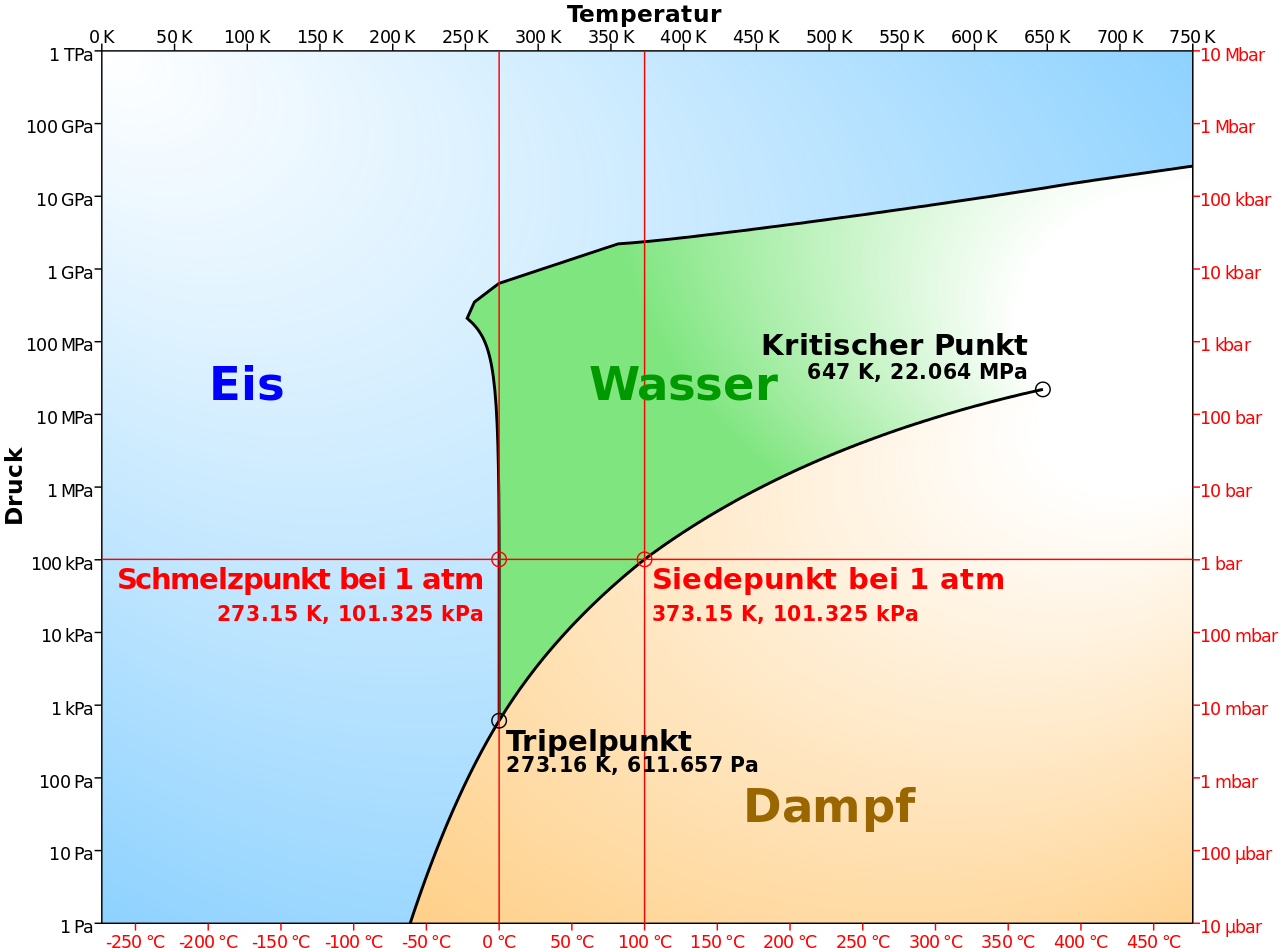
\includegraphics[width=\linewidth]{content/xx_test/Phase_diagram_of_water_simplified.svg.png}
	\caption{Vereinfachtes Phasendiagramm von Wasser \cite{TestCitation020}}
\end{figure}

\newpage

\subsection{Innerhalb eines Textes (Floating)}

\begin{wrapfigure}[14]{r}{0.33\textwidth}
	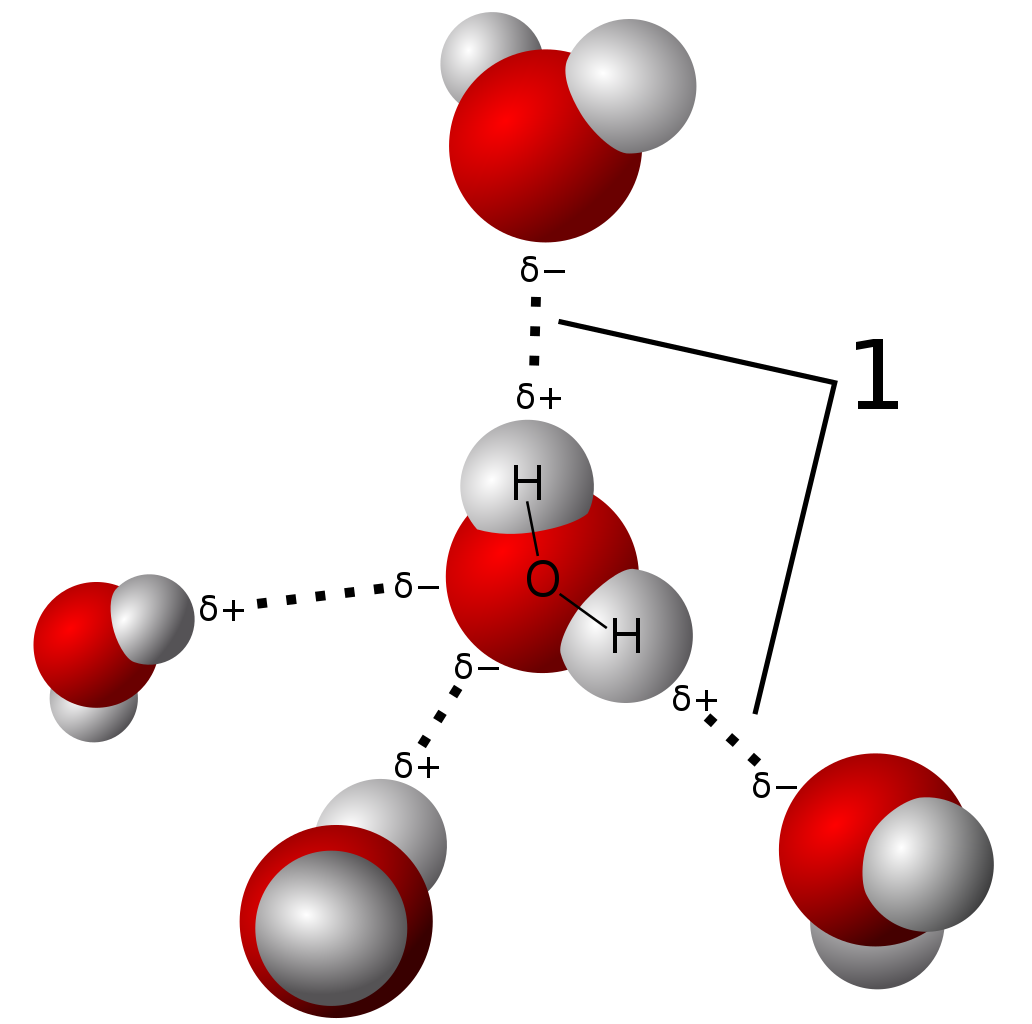
\includegraphics[width=\linewidth]{content/xx_test/1032px-3D_model_hydrogen_bonds_in_water.svg.png}
	\caption{Verkettung der Wassermoleküle \cite{TestCitation021}}
\end{wrapfigure}

Lorem ipsum dolor sit amet, consectetur adipiscing elit. Praesent eu risus a erat auctor bibendum. Morbi eget aliquet nisl. Aenean vestibulum elit sed arcu condimentum euismod. Nunc quis ipsum sed augue maximus molestie. Pellentesque condimentum elit vitae justo tincidunt elementum. Aliquam erat volutpat. Vestibulum feugiat auctor fringilla.

Cras non arcu ante. Donec faucibus lectus risus, ac sagittis risus malesuada pretium. Cras elementum quis turpis accumsan faucibus. Vestibulum vitae volutpat nisl, et sodales nunc. Etiam egestas at magna a commodo. Mauris sagittis suscipit tempus. Duis rhoncus nec ligula eget viverra. Maecenas eu nisl orci. Proin dignissim laoreet libero in interdum. Lorem ipsum dolor sit amet, consectetur adipiscing elit.

Sed fringilla lectus non elit convallis, non eleifend sem porta. Proin aliquet urna ultrices metus blandit ornare. Duis nec ultricies ligula, quis volutpat ante. Suspendisse non lacus mauris.

\begin{wrapfigure}[14]{o}{0.45\textwidth}
	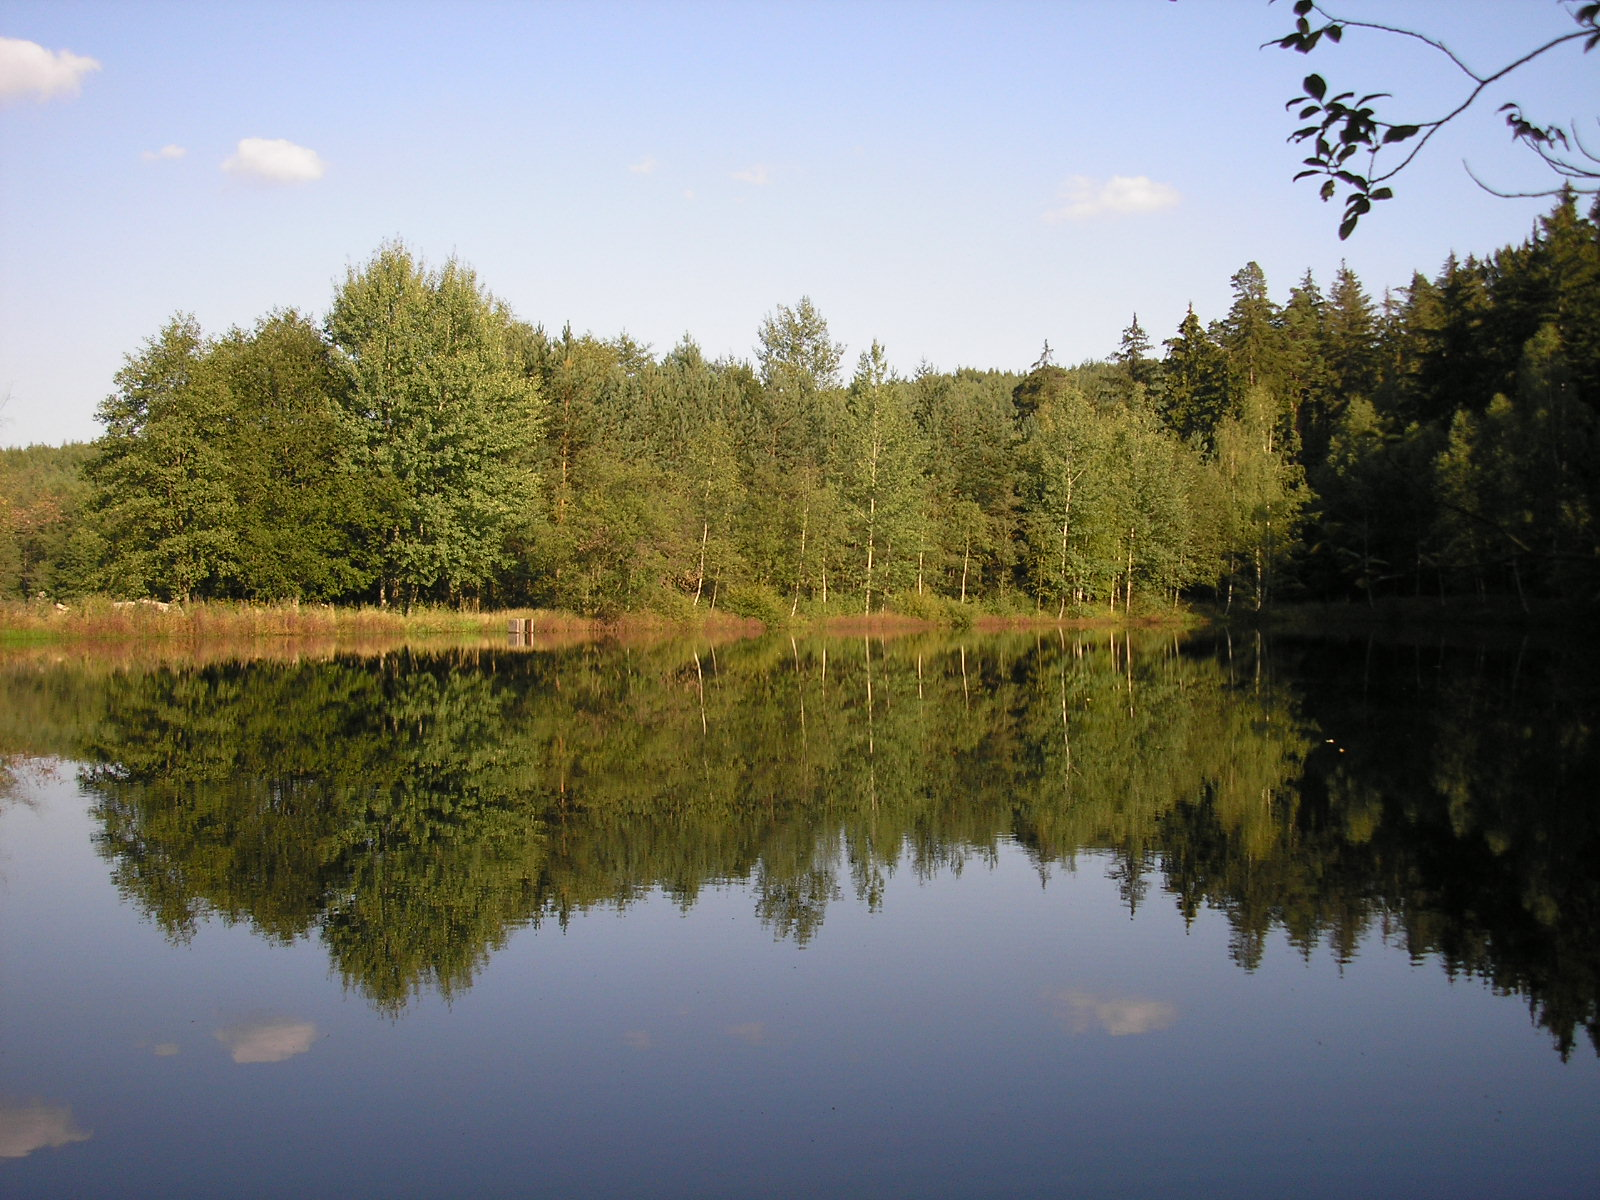
\includegraphics[width=\linewidth]{content/xx_test/Kleiner_Streichteich_Ilmenau.JPG}
	\caption{Spiegelung an der Wasseroberfläche \cite{TestCitation022}}
\end{wrapfigure}

Nullam quam diam, mattis non bibendum vel, iaculis sed leo. Phasellus condimentum auctor ante in mollis. Nullam rhoncus enim ac metus fermentum aliquam. Phasellus orci metus, tristique ac odio sed, fermentum faucibus mauris. Praesent vehicula risus aliquam nibh sodales, ac aliquam ante posuere. Praesent at semper sapien. In posuere augue vel tortor posuere rhoncus. Duis eget quam tempus diam posuere fringilla ut vitae lacus. Sed sagittis fringilla diam.

Suspendisse potenti. Ut pellentesque malesuada dolor vitae porta. Aliquam erat volutpat. Proin convallis mauris neque. Etiam et accumsan ex. Class aptent taciti sociosqu ad litora torquent per conubia nostra, per inceptos himenaeos. Suspendisse potenti. Cras ac magna enim. Praesent ultrices lacinia sem nec placerat. Sed tristique non sapien quis efficitur. Ut sit amet egestas metus. Mauris nec erat sodales, semper dolor eu, egestas justo. Ut sit amet urna ligula.

\section{Quellcode}

Der jeweilige Quellcode sollte mit Syntax-Highlighting versehen sein und im Quellcodeverzeichnis aufzufinden sein.

\subsection{Darstellung eines JavaScript Quellcodes (inline)}

\begin{lstlisting}[
  language = JavaScript,
     style = ES6,
   caption = Beispiel eines JavaScript Quellcodes (inline),
captionpos = b,
     label = lst:javascript-inline-example,
]
var fetch = require("node-fetch")

async function getCountries() {
  let res = await fetch("https://restcountries.eu/rest/v2/name/Indonesia?fullText=true")
  let json = await res.json()
  let code = json[0].alpha2Code
  let res2 = await fetch("http://country.io/phone.json")
  let json2 = await res2.json()
  console.log(json2[code])
}

getCountries()
\end{lstlisting}

\subsection{Darstellung eines JavaScript Quellcodes (importiert)}

\lstinputlisting[
  language = JavaScript,
     style = ES6,
   caption = Beispiel eines JavaScript Quellcodes (importiert),
captionpos = b,
     label = lst:javascript-import-example,
]{content/xx_test/import-example_javascript.js}

\subsection{Darstellung eines Java Quellcodes (inline)}

\begin{lstlisting}[
   caption = Beispiel eines Java Quellcodes (inline),
     label = lst:java-inline-example,
  language = java, 
     style = java-eclipse,
basicstyle = {\footnotesize\fontfamily{pcr}\selectfont}
]
	/*
	 * Main-Methode
	 */
	§§@LineAnnotation
	public class Main {
	  public static void main(%%@InlineAnnotation%% String[] args) {
	    System.out.println("Hallo Welt");
	  }
	}
\end{lstlisting}

\subsection{Darstellung eines Java Quellcodes (importiert)}

\lstinputlisting[
   caption = Beispiel eines Java Quellcodes (importiert),
     label = lst:java-import-example,
  language = java,
     style = java-eclipse,
basicstyle = {\footnotesize\fontfamily{pcr}\selectfont}
]{content/xx_test/import-example_java.js}
	
	\newpage{}
	
	\addcontentsline{toc}{chapter}{Eidesstattliche Erklärung}
	\chapter*{Eidesstattliche Erklärung}
	% siehe https://www.fh-dortmund.de/de/studi/studbuero/forms/medien/pruef_formulare_stud/FB4_Anmeldung_zur_BA_Thesis_2020-08-10.pdf

Hiermit versichere ich, dass ich die vorliegende Arbeit selbständig angefertigt und mich keiner fremden Hilfe bedient sowie keine anderen als die angegebenen Quellen und Hilfsmittel benutzt habe. Alle Stellen, die wörtlich oder sinngemäß veröffentlichten oder nicht veröffentlichten Schriften und anderen Quellen entnommen sind,habe ich als solche kenntlich gemacht. Diese Arbeit hat in gleicher oder ähnlicher Form noch keiner Prüfungsbehörde vorgelegen.
		
\vspace{4cm}
		
% bases on https://www.math.tugraz.at/~grabner/Masterarbeit-template.tex
\noindent
\begin{minipage}[h]{0.4\linewidth}
	Dortmund, am \dotfill\\
	\vspace*{2.5mm}
\end{minipage}
	\hspace*{0.1\linewidth}
	\begin{minipage}[h]{0.5\linewidth}
	\begin{center}
		\dotfill\\
		(Unterschrift)
	\end{center}
\end{minipage}
	
	\let\cleardoublepage\relax
	
	\newpage{}
	
	\addcontentsline{toc}{chapter}{Abkürzungsverzeichnis}
	
	\settowidth{\nomlabelwidth}{API}
	\printnomenclature{}
	
	\newpage{}
	
	\addcontentsline{toc}{chapter}{Abbildungsverzeichnis}
	
	\listoffigures
	
	\newpage{}
	
	\addcontentsline{toc}{chapter}{Tabellenverzeichnis}
	
	\listoftables
	
	\lstlistoflistings
	
	\newpage{}
	
	\bibliographystyle{alphadin}
	\bibliography{bib}
\end{document}
